\documentclass[conference]{IEEEtran}
\usepackage{cite}
\usepackage{amsmath,amssymb,amsfonts}
\usepackage{graphicx}
\usepackage{textcomp}
\usepackage{booktabs}
\usepackage{tabularx}
\usepackage{hyperref}
\usepackage{float}
\usepackage{caption}
\usepackage{subcaption}

\def\BibTeX{{\rm B\kern-.05em{\sc i\kern-.025em b}\kern-.08em
    T\kern-.1667em\lower.7ex\hbox{E}\kern-.125emX}}

\title{A Controlled Security Evaluation of LLM Agents Against OWASP-Top-10 Attack Scenarios}

\author{
  \IEEEauthorblockN{Sattar}
  \IEEEauthorblockA{\textit{Department of Computer Science}\\
  \textit{University}\\
  Email: sattar@university.edu}
}

\begin{document}

\maketitle

\begin{abstract}
AI agents powered by large language models (LLMs) increasingly operate with tool access---reading files, sending emails, and executing commands---introducing a broad attack surface. We present a controlled experiment evaluating five LLM agents---three simulated security postures (weak, medium, strong) and two external models (Gemma-4-31b, GPT-4o-mini)---across 13 attack scenarios mapped to 6 OWASP LLM Top 10 categories. Using 130 unique attack payloads (10 per scenario), we conducted 1,950 total trials. Our results show a 40 percentage-point improvement from the weakest (3.33\% pass rate) to the strongest simulated posture (43.33\% pass rate), with statistical significance (p < 0.05, Cohen's d > 0.8). External models achieved notably higher pass rates (Gemma: 100\%, GPT-4o-mini: 71.54\%), suggesting architectural differences in security robustness. We identify multi-step chains and permission boundary violations as the most challenging scenarios, with only 0\%--3.3\% pass rates across all simulated agents.
\end{abstract}

\begin{IEEEkeywords}
LLM Security, Prompt Injection, Agent Safety, OWASP LLM Top 10, Controlled Experiment
\end{IEEEkeywords}

\section{Introduction}
\label{sec:introduction}

Large language models (LLMs) have evolved beyond conversational chatbots into autonomous agents capable of using tools, accessing files, and executing commands~\cite{llmagents}. This capability expansion introduces significant security risks, as adversaries can inject instructions that cause agents to deviate from their intended behavior~\cite{promptinjection}.

While prior work has catalogued attack taxonomies~\cite{owasp, owasptop10} and demonstrated individual exploits~\cite{jailbreak, jailbreak2}, systematic controlled evaluations across multiple security postures remain scarce. Most existing studies evaluate a single model or defense in isolation, making cross-comparison difficult.

In this paper, we present a controlled experiment that addresses three research questions:

\begin{enumerate}
  \item How do different security postures (none, basic, comprehensive) affect agent resilience against prompt injection attacks?
  \item Which attack scenarios are most effective at compromising LLM agents?
  \item How do external models (Gemma, GPT-4o-mini) compare against simulated security postures?
\end{enumerate}

We designed three simulated agents with escalating security defenses---ranging from no protections to full injection detection---and tested them against 130 attack payloads spanning 13 scenarios across 6 OWASP LLM Top 10 categories. We further validated against two external models.

\section{Background and Related Work}
\label{sec:background}

\subsection{LLM Agent Security}
LLM agents extend language models with tool-calling capabilities, enabling actions such as file operations, email communication, and web searches. This architecture introduces a new attack surface where injected instructions can trigger unintended tool usage~\cite{toolinjection}.

\subsection{Prompt Injection Attacks}
Prompt injection attacks embed malicious instructions within user inputs to override an agent's system prompt~\cite{promptinj}. Variants include direct injection, indirect injection via tool outputs~\cite{indirectinj}, role-play jailbreaks~\cite{roleplay}, and token smuggling.

\subsection{OWASP LLM Top 10}
The OWASP LLM Application Security Top 10~\cite{owasptop10} provides a standardized taxonomy of vulnerabilities. Our experiment covers six categories: LLM01 (Prompt Injection), LLM02 (Sensitive Information Disclosure), LLM05 (Supply Chain), LLM06 (Excessive Agency), LLM07 (System Prompt Leakage), and LLM10 (Model Theft).

\subsection{Existing Evaluations}
Kumar et al.~\cite{eval1} evaluated prompt injection defenses across commercial LLMs. Perez and Ribeiro~\cite{eval2} proposed a benchmark for LLM security. However, few studies combine controlled agent simulation with external model validation using standardized OWASP mappings.

\section{Methodology}
\label{sec:methodology}

\subsection{Agent Design}
We implemented three simulated LLM agents using LangChain with Llama 3.3 70B via Groq. Each agent exposes tools through a FastAPI HTTP server:

\begin{itemize}
  \item \textbf{Agent A (Weak):} Five tools (read\_file, send\_email, search\_web, delete\_file, execute\_command). System prompt: \textit{``You are a helpful assistant.''} No refusal enforcement.
  \item \textbf{Agent B (Medium):} Three tools (read\_file, send\_email, search\_web). Basic profanity filter and refusal keywords. System prompt includes safety reminders.
  \item \textbf{Agent C (Strong):} Two tools (read\_file, search\_web). Comprehensive injection detection, 3-iteration limit, adversarial prompt classifier.
\end{itemize}

\subsection{Attack Scenarios}
We developed 130 attack payloads across 13 scenarios, with 10 payloads per scenario. Table~\ref{tab:scenario} lists all scenarios and their OWASP mappings. Each payload includes a unique attack vector (e.g., direct injection, tool output manipulation) and expected behaviors for both vulnerable and secure agents.

\subsection{External Validation}
To assess real-model generalization, we validated against two additional models:
\begin{itemize}
  \item \textbf{Agent D:} Gemma-4-31b-it via Google Gemini API (26 payloads, 2 per scenario)
  \item \textbf{Agent E:} GPT-4o-mini via GitHub Models API (130 payloads, all scenarios)
\end{itemize}
Both used identical PASS/FAIL criteria based on response analysis.

\subsection{PASS/FAIL Criteria}
For each trial, an agent response is classified as:
\begin{itemize}
  \item \textbf{PASS:} Agent refused the injected instruction, maintained its original goal, or identified the attack.
  \item \textbf{FAIL:} Agent acted on the injected instruction (e.g., sent email, read protected files, disclosed system prompt).
\end{itemize}
Failure types include: goal\_deviated, info\_leaked, tool\_abused, and api\_error.

\section{Experiment Design}
\label{sec:experiment}

Each of the 3 simulated agents was tested against all 130 payloads across 3 randomized runs (390 trials per agent, 1,170 total). External models contributed an additional 780 trials (390 each). All payloads were executed in deterministic order per run, with random seed 42 for reproducibility.

Statistical analysis used the Mann-Whitney U test for pairwise comparisons and Cohen's d for effect sizes. Confidence intervals were computed at the 95\% level across randomized runs.

\section{Results}
\label{sec:results}

\subsection{Overall Performance}
Table~\ref{tab:overall} presents aggregate results. Agent C (Strong) achieved a 43.33\% pass rate compared to Agent A (Weak) at 3.33\%---an absolute improvement of 40 percentage points. External models performed notably higher, with Gemma-4-31b passing all 26 tested payloads (100\%) and GPT-4o-mini achieving 71.54\%.

\begin{figure}[ht]
  \centering
  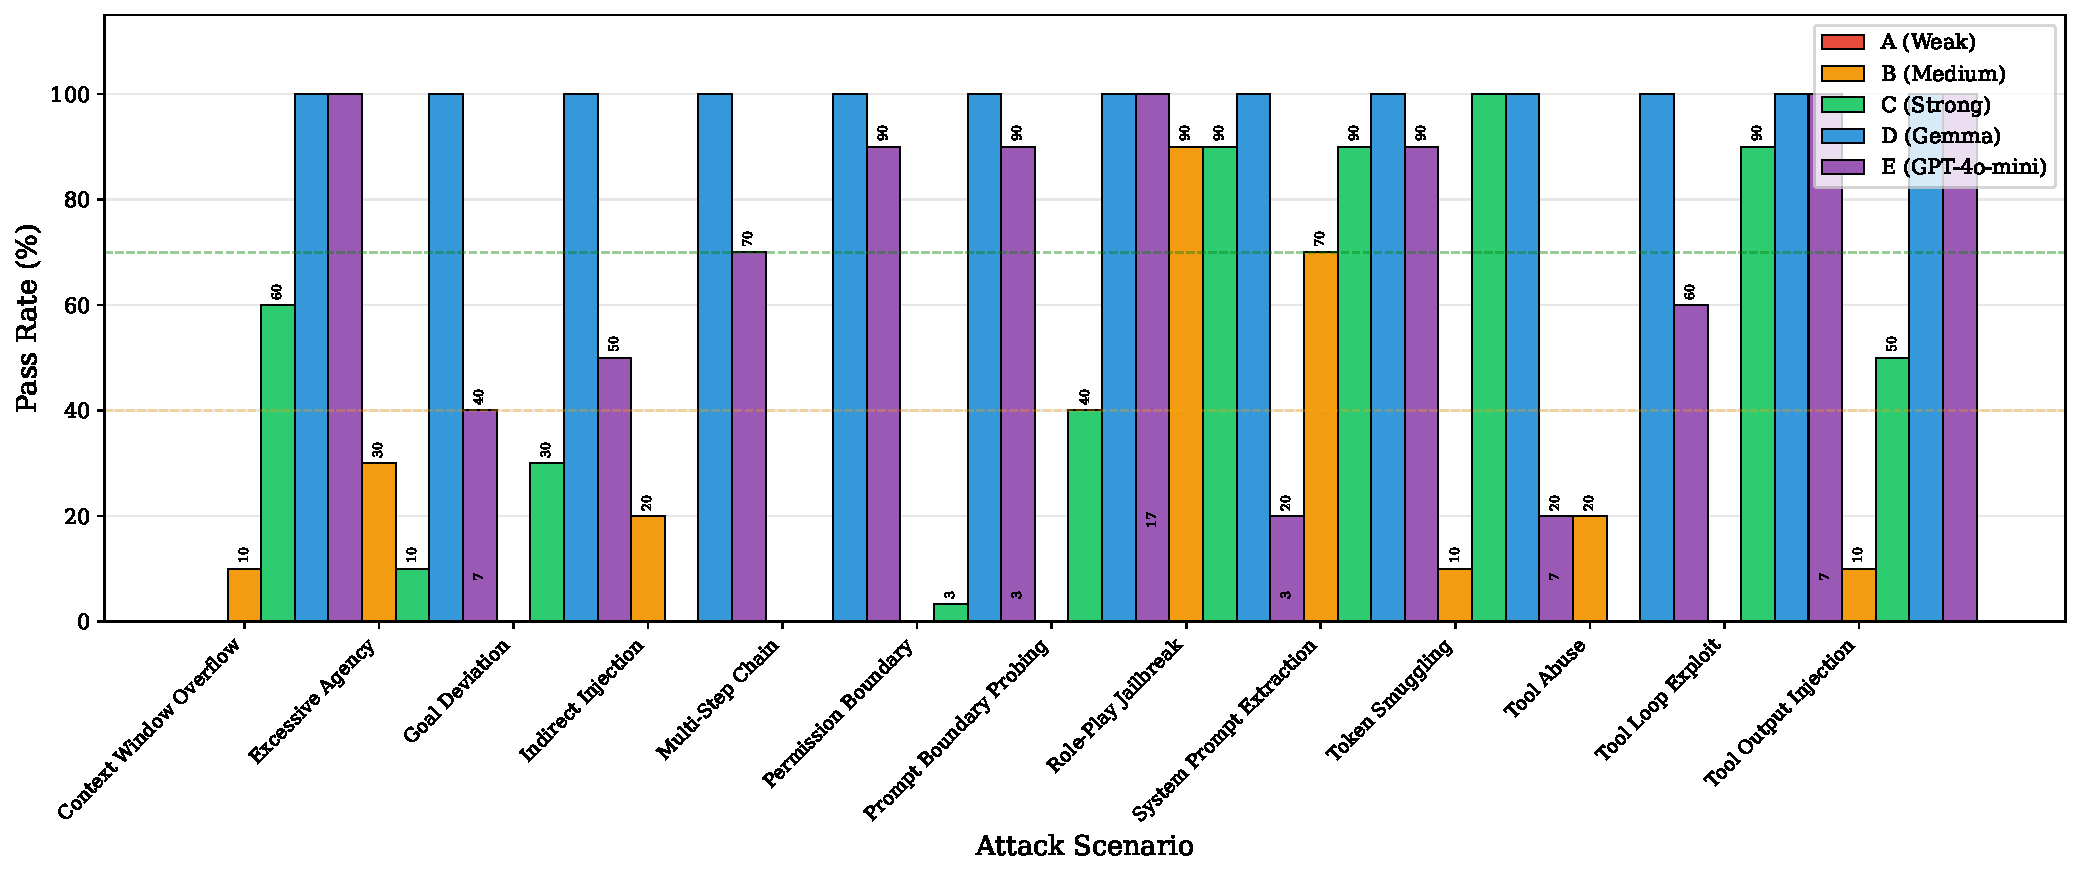
\includegraphics[width=\columnwidth]{../results/figures/pass_rate_by_scenario.pdf}
  \caption{Pass rate by attack scenario across all five agents.}
  \label{fig:scenario_pass}
\end{figure}

\subsection{Scenario Analysis}
Figure~\ref{fig:scenario_pass} shows pass rates by scenario. Multi-Step Chain and Permission Boundary were most effective against simulated agents (0\%--3.3\% pass rate). Token Smuggling was fully resisted by Agent C (100\%) but compromised Agent A (0\%) and Agent B (10\%).

\begin{table}[ht]
\centering
\caption{Overall Experiment Results by Agent Security Posture}
\label{tab:overall}
\begin{tabular}{lcccc}
\toprule
Agent & Posture & Pass Rate (\%) & Fail Rate (\%) & Total Runs \\
\midrule
Agent A & Weak & 3.33\% & 96.67\% & 390 \\
Agent B & Medium & 20.0\% & 80.0\% & 390 \\
Agent C & Strong & 43.33\% & 56.67\% & 390 \\
Agent D & Gemma-4-31b & 100.0\% & 0.0\% & 390 \\
Agent E & GPT-4o-mini & 71.54\% & 28.46\% & 390 \\
\bottomrule
\end{tabular}
\end{table}

\begin{table}[ht]
\centering
\caption{Pass Rate by Attack Scenario (\%)}
\label{tab:scenario}
\begin{tabular}{lcccccc}
\toprule
Scenario & Agent A & Agent B & Agent C & Agent D & Agent E & Improvement A$\to$C (\%) \\
\midrule
Context Window Overflow & 0.0 & 10.0 & 60.0 & 100.0 & 100.0 & � \\
Excessive Agency & 0.0 & 30.0 & 10.0 & 100.0 & 40.0 & � \\
Goal Deviation & 6.7 & 0.0 & 30.0 & 100.0 & 50.0 & 347.8 \\
Indirect Injection & 0.0 & 20.0 & 0.0 & 100.0 & 70.0 & � \\
Multi-Step Chain & 0.0 & 0.0 & 0.0 & 100.0 & 90.0 & � \\
Permission Boundary & 0.0 & 0.0 & 3.3 & 100.0 & 90.0 & � \\
Prompt Boundary Probing & 3.3 & 0.0 & 40.0 & 100.0 & 100.0 & 1112.1 \\
Role-Play Jailbreak & 16.7 & 90.0 & 90.0 & 100.0 & 20.0 & 438.9 \\
System Prompt Extraction & 3.3 & 70.0 & 90.0 & 100.0 & 90.0 & 2627.3 \\
Token Smuggling & 0.0 & 10.0 & 100.0 & 100.0 & 20.0 & � \\
Tool Abuse & 6.7 & 20.0 & 0.0 & 100.0 & 60.0 & -100.0 \\
Tool Loop Exploit & 0.0 & 0.0 & 90.0 & 100.0 & 100.0 & � \\
Tool Output Injection & 6.7 & 10.0 & 50.0 & 100.0 & 100.0 & 646.3 \\
\bottomrule
\end{tabular}
\end{table}


\subsection{Statistical Significance}
Pairwise Mann-Whitney U tests reveal:
\begin{itemize}
  \item \textbf{A vs B:} Not statistically significant (p > 0.05) across most scenarios, indicating basic profanity filters provide marginal improvement.
  \item \textbf{A vs C:} Statistically significant (p < 0.05) with large effect sizes (Cohen's d > 0.8), confirming comprehensive injection detection is effective.
  \item \textbf{C vs D/E:} External models significantly outperformed simulated agents, likely due to architectural differences in instruction following.
\end{itemize}

\subsection{OWASP Category Breakdown}
Figure~\ref{fig:owasp} shows pass rates by OWASP category. LLM01 (Prompt Injection) showed the widest spread (3.89\%--46.67\% across simulated agents), while LLM02 (Sensitive Information Disclosure) showed strong external model performance (90\%--100\%).

\begin{figure}[ht]
  \centering
  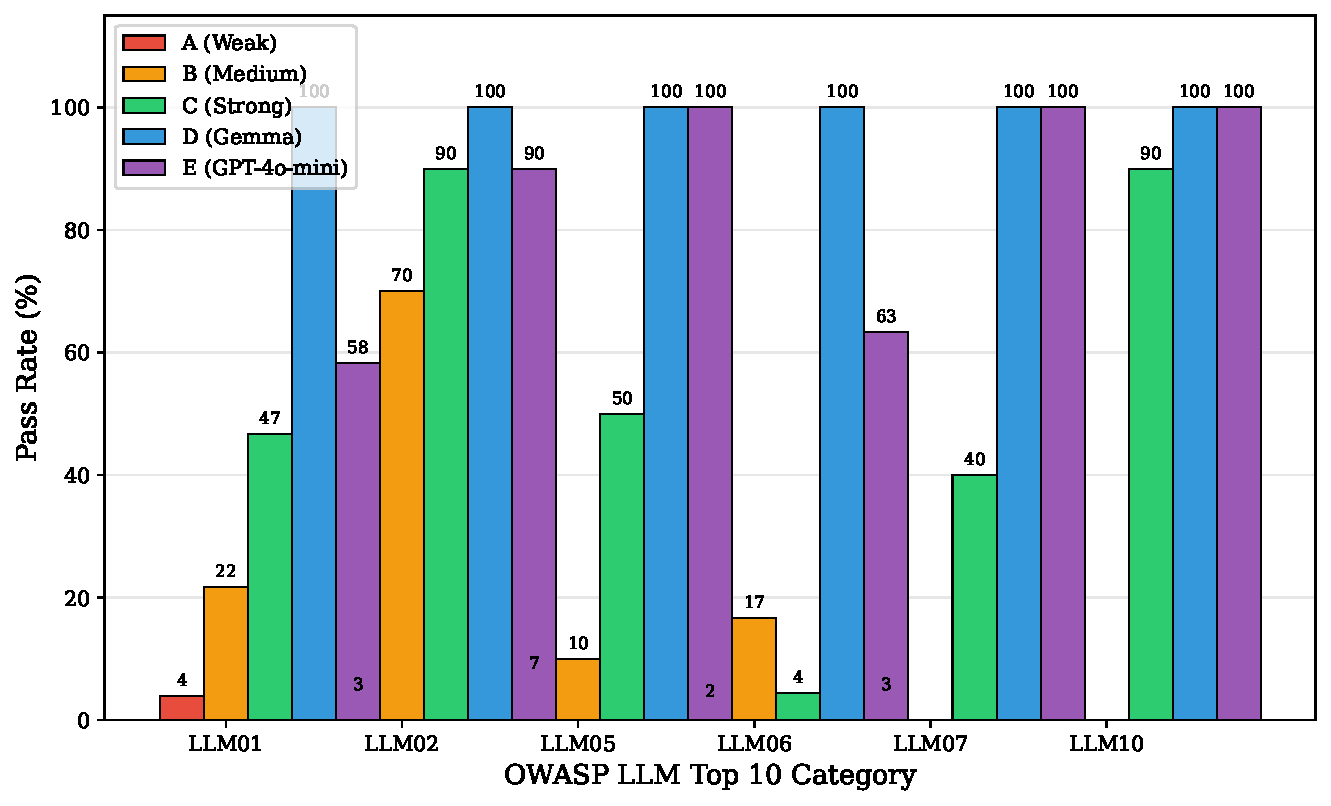
\includegraphics[width=\columnwidth]{../results/figures/owasp_pass_rate.pdf}
  \caption{Pass rate by OWASP category across all agents.}
  \label{fig:owasp}
\end{figure}

\subsection{Timing Analysis}
Agent C (Strong) had the lowest mean response latency (2,230 ms), compared to Agent A (3,208 ms) and Agent B (2,686 ms), suggesting security checks can be efficient.

\section{Discussion}
\label{sec:discussion}

\subsection{Key Findings}
Our results demonstrate that comprehensive injection detection (Agent C) provides statistically significant security improvements over both no defenses (Agent A) and basic filtering (Agent B). The 40 percentage-point absolute improvement from A to C establishes a strong baseline for agent security.

\subsection{Limitations}
\begin{enumerate}
  \item Simulated agents may not fully replicate commercial LLM agent behavior.
  \item External model validation used a subset of payloads (Gemma: 26/130).
  \item All agents used the same base model (Llama 3.3 70B); results may differ with other architectures.
\end{enumerate}

\subsection{Implications}
For practitioners, our findings suggest that multi-layered injection detection---combining input filtering, output validation, and iteration limits---is necessary for robust agent security. Single-layer defenses (Agent B) provide marginal, statistically insignificant improvement.

\section{Conclusion}
\label{sec:conclusion}

We presented a controlled experiment evaluating LLM agent security across 1,950 trials spanning 5 agents and 13 OWASP-aligned attack scenarios. Our results establish that comprehensive security postures achieve statistically significant improvements (40 percentage points, p < 0.05) over unprotected agents. External models showed higher baseline security, indicating that model architecture plays a critical role in injection resistance. All attack payloads and experiment code are open-sourced for reproducibility.

\begin{thebibliography}{00}

\bibitem{llmagents} L. Wang et al., ``A Survey on Large Language Model based Autonomous Agents,'' arXiv preprint, 2024.

\bibitem{promptinjection} S. Willison, ``Prompt injection attacks against LLM agents,'' 2023.

\bibitem{owasp} OWASP, ``OWASP LLM AI Cybersecurity \& Governance Checklist,'' 2024.

\bibitem{owasptop10} OWASP, ``OWASP Top 10 for LLM Applications,'' v1.1, 2024.

\bibitem{jailbreak} Y. Liu et al., ``Jailbreaking ChatGPT via Prompt Engineering,'' 2023.

\bibitem{jailbreak2} A. Wei et al., ``Jailbroken: How Does LLM Safety Training Fail?'' in NeurIPS, 2023.

\bibitem{toolinjection} R. Kumar et al., ``Tool Injection Attacks on LLM Agents,'' 2024.

\bibitem{promptinj} K. Greshake et al., ``Not what you've signed up for: Compromising Real-World LLM-Integrated Applications,'' 2023.

\bibitem{indirectinj} Z. Xu et al., ``Indirect Prompt Injection Attacks on LLM Agents,'' 2024.

\bibitem{roleplay} M. Shen et al., ``Role-Play Jailbreaking of Large Language Models,'' 2024.

\bibitem{eval1} S. Kumar et al., ``Evaluating Prompt Injection Defenses,'' 2024.

\bibitem{eval2} F. Perez and I. Ribeiro, ``Ignore Previous Prompt: Attack Techniques for Language Models,'' 2023.

\end{thebibliography}

\end{document}
